\documentclass[conference]{IEEEtran}
%\IEEEoverridecommandlockouts
\usepackage{cite}
\usepackage{amsmath,amssymb,amsfonts}
\usepackage{algorithmic}
\usepackage{graphicx}
\usepackage{textcomp}
\usepackage{xcolor}

\usepackage{lipsum}

\begin{document}

\title{Understanding the Mirai Botnet: A Summary}

\author{\IEEEauthorblockN{Ulysses Butler, Torey Clark, Thu Vo, Tung Thai}
\IEEEauthorblockA{\textit{CS 455 - Cybersecurity Fundamentals} \\
\textit{Truman State University}\\
Kirksville, MO \\
ub4782@truman.edu}
}

\maketitle

\section{Introduction}

In August of 2016, a server from a US bulletproof hosting service starting scanning computers. Shortly after this preliminary scan, the Marai botnet emerged. Within hours, it had infected hundreds of thousands of poorly secured IoT devices. In this paper, Zane Ma, et al. reverse engineer the malware and try to understand how it spread and what made it so effective. This botnet gained notoriety after being used to commit record smashing DDoS attacks. This botnet, and others that evolved from it, are believed to be responsible for high profile attacks on Krebs on Security, Dyn, OVH, and Lonestar Cell. Services provided by companies like Amazon, Twitter, GitHub, and Netflix were disrupted since they receive DNS services from Dyn. By the end of 2017, the botnet started to fade away and the creators were located by Krebs and the FBI.

\begin{figure}[b]
\centerline{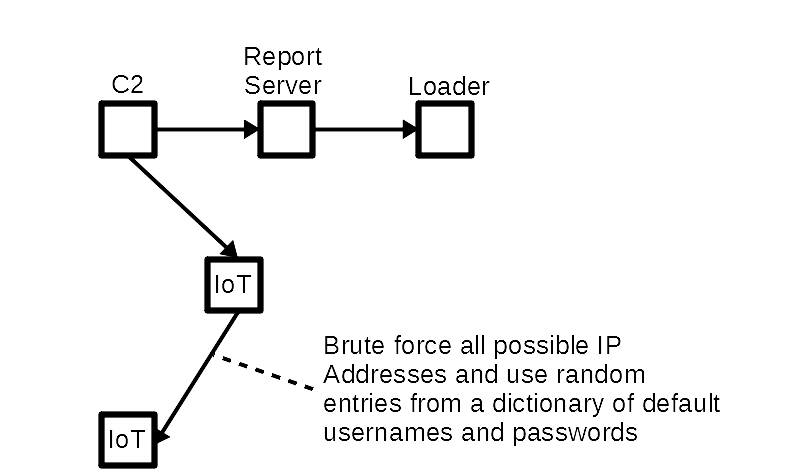
\includegraphics[width=0.45\textwidth]{../fig1.png}}
\caption{A bot would start scanning other devices to infect}
\label{scan}
\end{figure}

\section{Spreading Marai}

On August 1st, 2016, servers owned by DataWagon began a scan that lasted about two hours. About 40 minutes later, it starting infecting devices. Within a minute, over 800 devices were infected. After 10 minutes, they had over 11,000 devices with the malware. This kept increasing with a doubling rate of about 75 minutes until it stabilized with 100k to 200k machines. Once infected, a device would begin to scan other devices. It would check every IPv4 address for open ports running services like SSH, FTP, and Telnet. It carried a blacklist of IP addresses associated with the US Department of Defense and a number of major corporations. This allowed it to go largely undetected. Furthermore, these entites have the resources to properly study and defeat the botnet, so avoiding them gave Marai a better chance of spreading. Once it found a device to infect, it would start brute forcing the credentials. It did this using a small dictionary of anywhere from 60 to about 200 default manufacturer credentials as seen in fig.~\ref{scan}. 

 \begin{figure}[t]
\centerline{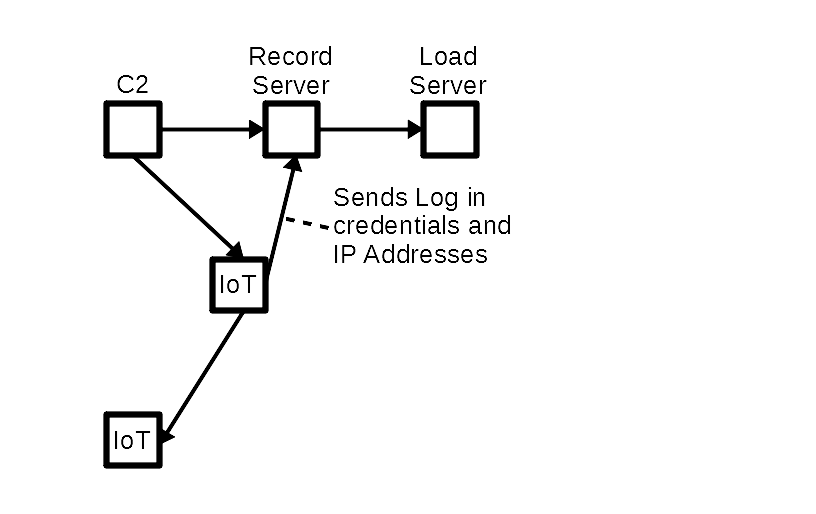
\includegraphics[width=0.45\textwidth]{../fig2.png}}
\caption{The IP address and credentials are then sent to the report server}
\label{report}
\centerline{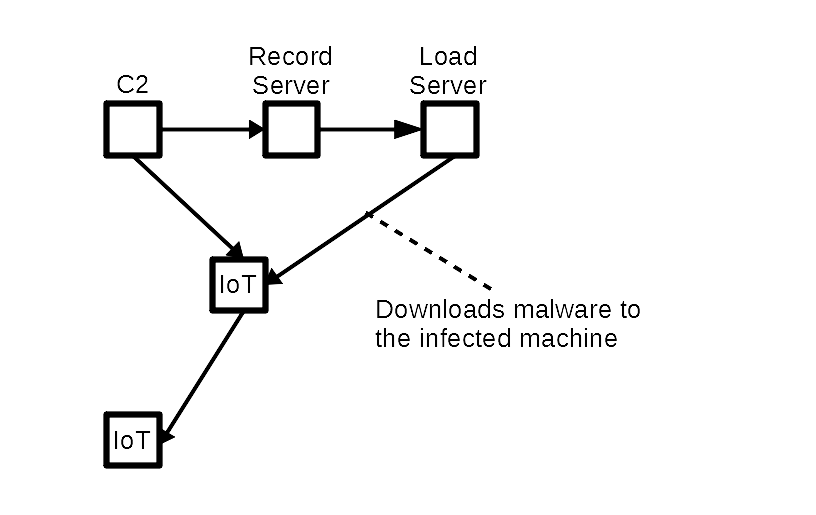
\includegraphics[width=0.45\textwidth]{../fig3.png}}
\caption{The report server dispatches the loader program to install the binary}
\label{loader}
\end{figure}

Once the bot figured out what the username and password were, this information was sent back to a report server, as seen in fig.~\ref{report}. This server would then send the information to dispatch the loader program. The loader program would then log in to the newly cracked machine and download an architecture specific binary. This binary would then be run. Once the program was loaded into memory, it would delete the binary. This made it much more difficult to study. It would then obscure information about its process to make it harder to detect, shown in fig.~\ref{loader}.

\section{Internet of Things Devices}

This botnet was notable for targeting devices in the Internet of Things (IoT). This mainly consists of small, embedded devices. This includes things like cameras, printers, routers, and DVRs. That being said, the Internet of Things doesn't include devices like personal computers, servers, and cell phones. These devices are much more powerful, but also much more secure. Manufactures of IoT devices often neglect good security practice. Many of these device ship with the same username and password. Often, they use common credentials like \verb|admin|, \verb|password|, and the name of the company or product. The author of Mirai took advantage of this fact. They were able to include this relatively small list of common credentials in their dictionary. This allowed the botnet to gain access to such a large number of devices despite having such a small dictionary. This lack of good security practice by these manufactures made all of their products vulnerable to these unsophisticated attack. This vulnerability, combined with how prevalent and widespread these devices were, made an especially potent combination.

\section{Methodology}

The researchers used a number of methods to track the spread of Mirai and study how it worked. Network telescopes are systems that allow authorities to monitor large, unusual activity on the internet. Researchers were able to use information from these network telescopes to study the spread of Mirai. They monitored the large number of requests to unusual IPs to gain an idea of what machines were being scanned and were able to spot DDoS attacks by monitoring the sudden flood of \verb|SYN| packets to a target. They attempted scanning infected device and used telnet honeypots to learn how Mirai operated. The honeypots are machines that look like vulnerable IoT devices to anyone scanning them. When the botnet tried to download binaries on the honeypots, they would log all of the information. Using this method, the researchers were able to acquire some of the actual binaries Mirai used. These were then reverse engineered. Finally, they studied the DNS records and the attack commands to try to figure out who was controlling the botnet and who the targets were.

\section{Open Source}

On September 30, 2016, the source code was release on \verb|hackerforums.net| by a user named Anna-senpai. This allowed other hackers to create copy cat attacks. Following the release was a wave of new strains of the Mirai botnets. These botnets started to evolve and compete. These new strains contained modified credential lists, and used more advanced exploits. They would try to disable competing strains of the malware that were operating on the same device and close ports that could be used for future vectors of attack. This also made it harder to study the malware and scan infected devices. 

\section{Defending Against Future Attacks}

With its overwhelming power and devastation, Mirai served as a wake up call to security experts. This authors of this paper recommends a number of improvements manufactures can make to prevent similar attacks from occurring again in the future. IoT device manufactures can randomize the default passwords, making it harder to brute force into them, stunting growth of the botnet. They could close the ports to unused services like Telnet and SSH. They also recommend creating infrastructure to update the hardware. This way, the companies would be able to create future patches as needed.

\section{Conclusion}

The Mirai botnet was responsible for some of the largest and highest profile DDoS attacks ever recorded. That being said, it was a relatively simple and unsophisticated program that was able to brute force into machines using a small dictionary. It was able to do this because of the rampant use of poor security practice by IoT device manufactures. After Mirai, security experts have a better idea of what reforms can be made to prevent similar attacks in the future. Though we'll likely never be able to escape the threat of a DDoS attack, we can take steps towards mitigating their damage.

\bibliographystyle{IEEEtran}
\bibliography{ref}

\end{document}
